\setauthor{Antonio Kuvac}
\section{Start-Screen}
\setauthor{Antonio Kuvac}

Wenn die App geöffnet wird, erscheint zunächst der Startbildschirm.

\begin{figure}[H]
        \centering
        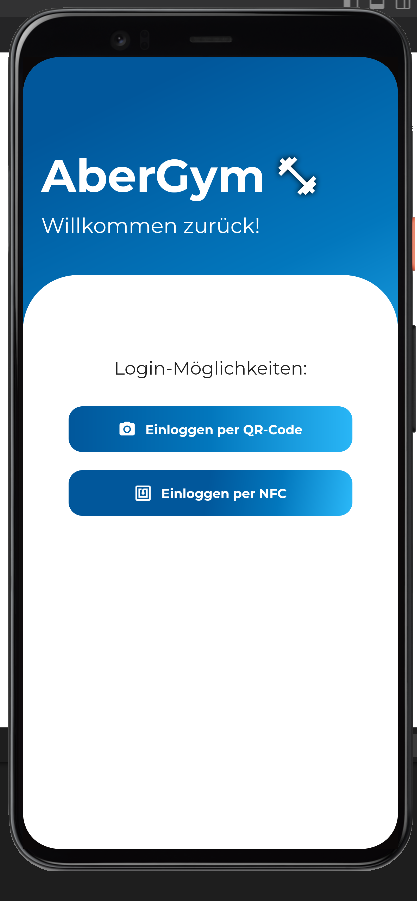
\includegraphics[scale=0.3]{pics/Start-Screen.png}
        \caption{Start-Screen}
    \end{figure}

Dieser wurde wie folgt implementiert:

\begin{lstlisting}[caption=Start-Screen Packages,label=lst:impl:frontend:packages]
    import 'package:abergymmobile/AGM.Animations/FadeAnimation.dart';
    import 'package:abergymmobile/AGM.Login/NFC.dart';
    import 'package:abergymmobile/AGM.Login/QrCode.dart';
    import 'package:google_fonts/google_fonts.dart';
    import 'package:flutter/foundation.dart';
    import 'package:flutter/material.dart';
    import 'package:flutter/services.dart';
\end{lstlisting}

Der Code importiert verschiedene Pakete, um das Layout und die Funktionen der Anwendung zu erstellen. Dazu gehören Google Fonts für benutzerdefinierte Schriftarten und Flutter-Pakete für Widgets und das Material Design.
\pagebreak

\begin{lstlisting}[caption= main-Funktion,label=lst:impl:frontend:main]
    Future<void> main() async {
        WidgetsFlutterBinding.ensureInitialized();
        SystemChrome.setEnabledSystemUIMode(SystemUiMode.manual, overlays: []);
        debugDefaultTargetPlatformOverride = null;
        runApp(const MaterialApp(
        debugShowCheckedModeBanner: false,
        home: LoginPage(),
        ));
        }
\end{lstlisting}

Die main-Funktion initialisiert die Flutter-App und startet sie. Sie setzt den System-UI-Modus und entfernt das Debug-Banner. Schließlich wird die LoginPage als Startseite festgelegt.
\newline

\begin{lstlisting}[caption=Login-Seite,label=lst:impl:frontend:login-seite]
    class LoginPage extends StatelessWidget {
const LoginPage({super.key});

@override
Widget build(BuildContext context) {
return Scaffold(
...
);
}
}
\end{lstlisting}

Das LoginPage-Widget erstellt die Login-Seite. Diese Seite ist in mehrere Abschnitte unterteilt, die im Folgenden erläutert werden.
\newline

\begin{lstlisting}[caption=Layout und Hintergrundfarbe,label=lst:impl:frontend:layout]
    decoration: BoxDecoration(
        gradient: LinearGradient(
        begin: Alignment.topCenter,
        colors: [
        Colors.lightBlue[900]!,
        Colors.lightBlue[800]!,
        Colors.lightBlue[400]!,
        ],
        ),
        ),
\end{lstlisting}

Mit LinearGradient wird ein linearer Farbverlauf von Hellblau bis Dunkelblau erstellt der von oben nach unten verläuft(begin: Allignment.topCenter).
\pagebreak

\begin{lstlisting}[caption=Logo und Willkommensnachricht,label=lst:impl:frontend:layout]
    children: <Widget>[
        FadeAnimation(
          1,
          Row(
            children: <Widget>[
              Text(
                "AberGym",
                style: GoogleFonts.montserrat(
                  color: Colors.white,
                  fontSize: 50,
                  fontWeight: FontWeight.bold,
                ),
              ),
              const SizedBox(width: 10),
              const Icon(
                Icons.fitness_center,
                color: Colors.white,
                size: 50,
                shadows: <Shadow>[
                  Shadow(
                    color: Colors.black,
                    blurRadius: 20.0,
                  )
                ],
              )
            ],
          ),
        ),
        const SizedBox(height: 10),
        FadeAnimation(
          1.3,
          Text(
            "Willkommen zurueck!",
            style: GoogleFonts.montserrat(
              color: Colors.white,
              fontSize: 23,
            ),
          ),
        ),
      ],
\end{lstlisting}

Der Code erstellt das AberGym-Logo und die Willkommensnachricht mit Hilfe von \texttt{FadeAnimation}, \texttt{Text}- und \texttt{Icon}-Widgets.
\pagebreak

\begin{lstlisting}[caption=QR-Code Schaltfläche,label=lst:impl:frontend:qrcode]
FadeAnimation(
1.6,
GestureDetector(
onTap: () {
Navigator.push(
context,
MaterialPageRoute(
builder: (context) => const QRCodePage(),
),
);
},
child: Container(
height: 50,
margin: const EdgeInsets.symmetric(horizontal: 20),
decoration: BoxDecoration(
gradient: LinearGradient(
begin: Alignment.centerLeft,
colors: [
Colors.lightBlue[900]!,
Colors.lightBlue[800]!,
Colors.lightBlue[400]!,
],
),
color: Colors.lightBlue,
borderRadius: BorderRadius.circular(15),
),
child: Row(
mainAxisAlignment: MainAxisAlignment.center,
children: [
const Icon(
Icons.camera_alt,
color: Colors.white,
size: 20,
),
const SizedBox(width: 10),
Text(
"Einloggen per QR-Code",
style: GoogleFonts.montserrat(
color: Colors.white,
fontWeight: FontWeight.bold,
),
),
],
),
),
),
),
\end{lstlisting}

Diese Schaltfläche ermöglicht dem Benutzer*der Benutzerin, sich per QR-Code einzuloggen. Sie verwendet \texttt{FadeAnimation}, \texttt{GestureDetector}, \texttt{Container} und \texttt{Row}-Widgets, um das Layout und die Funktionen der Schaltfläche zu erstellen. Beim Tippen auf die Schaltfläche wird der Benutzer*die Benutzerin zur \texttt{QRCodePage} weitergeleitet.
\pagebreak

\begin{lstlisting}[caption=NFC Schaltfläche,label=lst:impl:frontend:qrcode]
FadeAnimation(
1.7,
GestureDetector(
onTap: () {
Navigator.push(
context,
MaterialPageRoute(
builder: (context) => const NFC(),
),
);
},
child: Container(
height: 50,
margin: const EdgeInsets.symmetric(horizontal: 20),
decoration: BoxDecoration(
gradient: LinearGradient(
begin: Alignment.topCenter,
colors: [
Colors.lightBlue[900]!,
Colors.lightBlue[800]!,
Colors.lightBlue[400]!,
],
),
color: Colors.lightBlue,
borderRadius: BorderRadius.circular(15),
),
child: Row(
mainAxisAlignment: MainAxisAlignment.center,
children: [
const Icon(
Icons.nfc,
color: Colors.white,
size: 20,
),
const SizedBox(width: 10),
Text(
"Einloggen per NFC",
style: GoogleFonts.montserrat(
color: Colors.white,
fontWeight: FontWeight.bold,
),
),
],
),
),
),
),
\end{lstlisting}

Diese Schaltfläche ermöglicht dem Benutzer*der Benutzerin, sich per NFC einzuloggen. 
Ähnlich wie bei der QR-Code-Schaltfläche verwendet sie \texttt{FadeAnimation}, \texttt{GestureDetector}, \texttt{Container} und \texttt{Row}-Widgets, 
um das Layout und die Funktionen der Schaltfläche zu erstellen. Beim Tippen auf die Schaltfläche wird der Benutzer*die Benutzerin zur \texttt{NFC}-Seite weitergeleitet.
\newpage

\section{Login}
Um sich einzuloggen gibt es zwei Varianten. Entweder man loggt sich mithilfe eines QR-Codes ein oder mit NFC.

\subsection{QR-Code Login}

Die QR-Code-Funktion ermöglicht es Benutzer*innen, sich mit einem personalisierten QR-Code einzuloggen.

\begin{figure}[H]
    \centering
    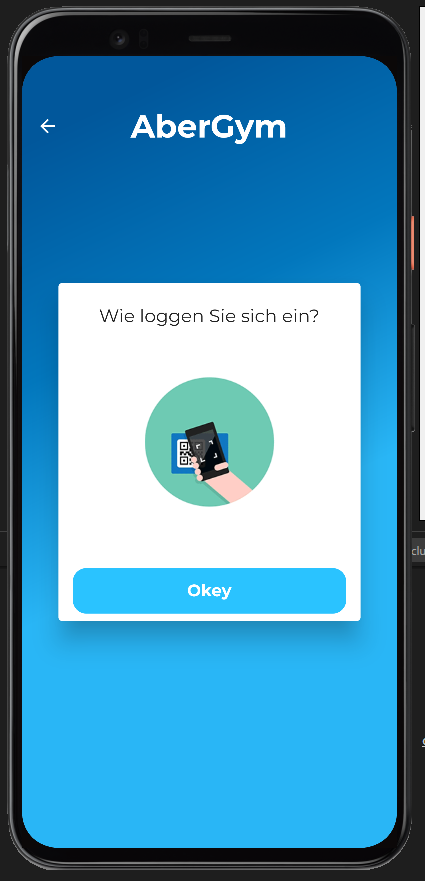
\includegraphics[scale=0.3]{pics/QRCodetutorial.png}
    \caption{QR-CodeTutorial}
\end{figure}
\begin{figure}[H]
    \centering
    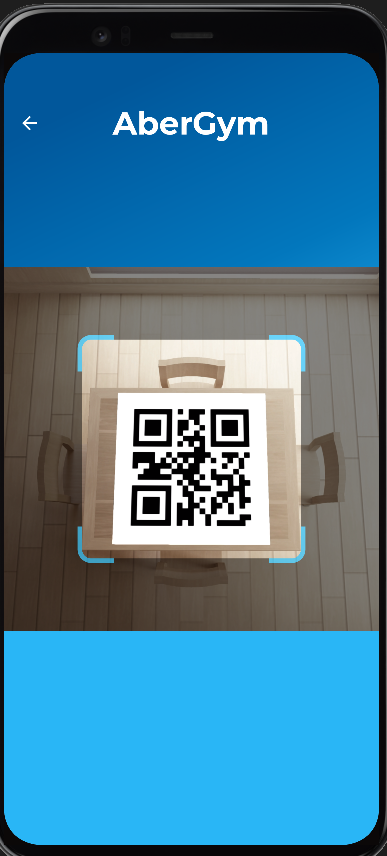
\includegraphics[scale=0.3]{pics/QR-CodeCamera.png}
    \caption{QR-Code auf Kamera}
\end{figure}
\pagebreak
\begin{lstlisting}[caption=QR-Code Seite erstellen,label=lst:impl:frontend:qrcode]
import 'package:qr_code_scanner/qr_code_scanner.dart';
import 'package:shared_preferences/shared_preferences.dart';

class QRCodePage extends StatefulWidget {
const QRCodePage({super.key});

@override
State<QRCodePage> createState() => _QRCodePageState();
}

class _QRCodePageState extends State<QRCodePage> {
final Color darkgrey = const Color.fromRGBO(37, 37, 50, 1);
final Color lightblue = const Color.fromARGB(255, 42, 195, 255);
bool showScanRect = false;
final GlobalKey qrKey = GlobalKey(debugLabel: 'QR');
Barcode? result;
QRViewController? controller;
bool logintrue = false;
String name = "";
bool _shouldNavigate = false;
\end{lstlisting}

Der Code beginnt mit dem Importieren der erforderlichen Pakete und dem Erstellen der \texttt{QRCodePage} StatefulWidget-Klasse. Der Zustand der Seite wird in der \texttt{QRCodePageState} Klasse verwaltet. Hier werden einige Variablen deklariert, wie zum Beispiel Farben, Zustände und der QRViewController.



\pagebreak
\begin{lstlisting}[caption=QR-Code Seitenstruktur,label=lst:impl:frontend:qrcode]
@override
Widget build(BuildContext context) {
return Scaffold(
extendBodyBehindAppBar: true,
appBar: AppBar(
title: Text(
'AberGym',
style: GoogleFonts.montserrat(
fontSize: 35,
color: Colors.white,
fontWeight: FontWeight.bold,
),
),
backgroundColor: Colors.transparent,
centerTitle: true,
elevation: 0,
),
body: Container(
width: double.infinity,
decoration: BoxDecoration(
gradient: LinearGradient(
begin: Alignment.topCenter,
colors: [
Colors.lightBlue[900]!,
Colors.lightBlue[800]!,
Colors.lightBlue[400]!,
],
),
),
child: Column(
mainAxisAlignment: MainAxisAlignment.center,
children: [
!showScanRect
? AlertDialog(
title: Text('Wie loggen Sie sich ein?',
textAlign: TextAlign.center,
style: GoogleFonts.getFont('Montserrat')),
content: Image.asset('assets/images/qrcode.gif'),
actions: [
GestureDetector(
child: Center(
child: Container(
width: 300,
height: 50,
decoration: BoxDecoration(
color: const Color.fromARGB(255, 42, 195, 255),
borderRadius: BorderRadius.circular(15),
),
child: Row(
mainAxisAlignment: MainAxisAlignment.center,
children: [
Text(
'Okey',
style: GoogleFonts.montserrat(
fontSize: 18,
color: Colors.white,
fontWeight: FontWeight.bold,
),
),
],
),
),
),
onTap: () {
setState(() {
showScanRect = true;
});
},
),
],
)
: SizedBox(
height: 400,
width: double.infinity,
child: _buildQrView(context),
),
],
),
),
);
}
\end{lstlisting}

In der \texttt{build}-Methode wird die Seitenstruktur der \texttt{QRCodePage} erstellt. Hier wird ein \texttt{Scaffold}-Widget verwendet, um die Hauptstruktur der Seite zu erzeugen. In der Mitte der Seite wird eine Bedingung geprüft, um entweder einen AlertDialog anzuzeigen, der Benutzer*innen darüber informiert, wie sie sich einloggen können, oder den QR-Code-Scanner anzuzeigen.
\linebreak
\begin{lstlisting}[caption=QR-Code Scanner erstellen,label=lst:impl:frontend:qrcode]
Widget _buildQrView(BuildContext context) {
var scanArea = (MediaQuery.of(context).size.width < 400 ||
MediaQuery.of(context).size.height < 400)
? 150.0
: 250.0;

return QRView(
key: qrKey,
onQRViewCreated: _onQRViewCreated,
overlay: QrScannerOverlayShape(
borderColor: lightblue,
borderRadius: 10,
borderLength: 30,
borderWidth: 10,
cutOutSize: scanArea),
);
}
\end{lstlisting}

Die \texttt{buildQrView}-Methode erstellt das QR-Code-Scanner-Widget. Das QRView-Widget erhält die Größe des Scanbereichs basierend auf der Bildschirmgröße und erstellt das Widget mit den angegebenen Design-Parametern.

\begin{lstlisting}[caption=QR-Code-Scanner Controller,label=lst:impl:frontend:qrcode]
void _onQRViewCreated(QRViewController controller) {
this.controller = controller;
controller.scannedDataStream.listen((scanData) {
setState(() {
result = scanData;
checkUser(result?.code);
});
if (_shouldNavigate) {
controller.dispose();
Navigator.of(context).pushReplacement(
MaterialPageRoute(builder: (context) => WelcomeSplashPage(name)));
}
});
}
\end{lstlisting}

Die \texttt{onQRViewCreated}-Methode wird aufgerufen, wenn das QRView-Widget erstellt wurde. Diese Methode initialisiert den \texttt{QRViewController} und hört auf den Datenstrom des gescannten QR-Codes. Wenn ein QR-Code gescannt wurde, wird die \texttt{checkUser} Methode aufgerufen, um die Benutzer*innen-Informationen abzurufen und die Seite zu navigieren, falls der Benutzer*die Benutzerin erfolgreich identifiziert wurde.

\begin{lstlisting}[caption=Datenbankabfrage QR-Code,label=lst:impl:frontend:qrcode]
Future<void> checkUser(String? qrCardId) async {
IResultSet result;

final conn = await MySQLConnection.createConnection(

);

await conn.connect();
result = await conn.execute(
"SELECT first_name, last_name FROM Person WHERE card_id = :card_id",
{"card_id": qrCardId},
);

for (final row in result.rows) {
setState(
() {
String? firstName = "";
String? lastName = "";
firstName = row.colAt(0);
lastName = row.colAt(1);
name = "$firstName $lastName";
},
);
}
final prefs = await SharedPreferences.getInstance();
if (name.isEmpty == false) {
setState(() {
_shouldNavigate = true;
logintrue = true;
prefs.setBool('login', logintrue);
prefs.setString('key', name);
});
}

await conn.close();
}
\end{lstlisting}

Die \texttt{checkUser}-Methode überprüft, ob der gescannte QR-Code mit einer gültigen Benutzerinnen-ID übereinstimmt, indem sie eine Datenbankabfrage durchführt. Sie verwendet die \texttt{MySQLConnection}-Klasse, um eine Verbindung zur Datenbank herzustellen, und führt eine SQL-Abfrage aus, um den Vornamen und Nachnamen des Benutzersin basierend auf der QR-Code-ID abzurufen. Wenn die Abfrage erfolgreich ist, wird der Name des Benutzers*in gespeichert und der Anmeldestatus in den \texttt{SharedPreferences} aktualisiert. Schließlich wird die Verbindung zur Datenbank geschlossen.

\pagebreak

\subsection{NFC Login}

Die NFC-Funktion ermöglicht es Benutzer*innen, sich mit einer Chipkarte wie einer Fitness-Mitgliedskarte einzuloggen.


\begin{lstlisting}[caption=NFC Package und State,label=lst:impl:frontend:qrcode]
import 'package:nfc_manager/nfc_manager.dart';

class NFC extends StatefulWidget {
const NFC({super.key});

@override
State<NFC> createState() => _NFCState();
}

class _NFCState extends State<NFC> {
bool _nfcEnabled = false;
ValueNotifier<dynamic> result = ValueNotifier(null);
final Color darkgrey = const Color.fromRGBO(37, 37, 50, 1);
final Color lightblue = const Color.fromARGB(255, 42, 195, 255);

@override
void initState() {
super.initState();
_checkNfcStatus();
}
}
\end{lstlisting}

Zunächst werden die erforderlichen Pakete importiert, insbesondere das \texttt{nfcmanager} Paket. Die \texttt{NFC}-Klasse erbt von \texttt{StatefulWidget}, und der zugehörige \texttt{State} wird in der \texttt{NFCState}-Klasse definiert. In \texttt{NFCState} werden die initialen Zustände und Farben gesetzt, und die Methode \texttt{initState} wird überschrieben, um den NFC-Status beim Start der Anwendung zu überprüfen.
\newline

\begin{lstlisting}[caption=NFC Status überprüfen,label=lst:impl:frontend:qrcode]
void _checkNfcStatus() async {
bool nfcEnabled = await NfcManager.instance.isAvailable();
setState(() {
_nfcEnabled = nfcEnabled;
});
}
\end{lstlisting}

Die Methode \texttt{checkNfcStatus} überprüft, ob NFC auf dem Gerät verfügbar und aktiviert ist. Mithilfe der \texttt{NfcManager}-Instanz wird die Methode \texttt{isAvailable} aufgerufen, um den NFC-Status abzurufen. Der ermittelte Status wird dann im \texttt{nfcEnabled} Attribut gespeichert.
\pagebreak

\begin{lstlisting}[caption=NFC Tag scannen,label=lst:impl:frontend:qrcode]
void _startScan() {
NfcManager.instance.startSession(onDiscovered: (NfcTag tag) async {
result.value = tag.data;
NfcManager.instance.stopSession();
});
}
\end{lstlisting}

Die Methode \texttt{startScan} startet die NFC-Session und wartet auf das Entdecken eines NFC-Tags. Sobald ein Tag entdeckt wird, wird die \texttt{onDiscovered}-Funktion aufgerufen, die die Daten des NFC-Tags in der \texttt{result}-Variable speichert und die Session beendet.
\newline
\begin{lstlisting}[caption=NFC Widget erstellen,label=lst:impl:frontend:qrcode]
    @override
    Widget build(BuildContext context) {
    return Scaffold(
    extendBodyBehindAppBar: true,
    appBar: AppBar(
    title: Text(
    'AberGym',
    style: GoogleFonts.montserrat(
    fontSize: 35,
    color: Colors.white,
    fontWeight: FontWeight.bold,
    ),
    ),
    backgroundColor: Colors.transparent,
    centerTitle: true,
    elevation: 0,
    ),
    backgroundColor: darkgrey,
    body: Container(
    decoration: BoxDecoration(
    gradient: LinearGradient(
    begin: Alignment.topCenter,
    colors: [
    Colors.lightBlue[900]!,
    Colors.lightBlue[800]!,
    Colors.lightBlue[400]!,
    ],
    ),
    ),
    child: _nfcEnabled
    ? Column(
    mainAxisAlignment: MainAxisAlignment.center,
    children: [
    Text(
    "Bitte halten Sie Ihre Fitnesskarte zum Handy, um die Karte zu scannen!",
    style: GoogleFonts.montserrat(
    color: Colors.white,
    fontWeight: FontWeight.bold,
    fontSize: 25,
    ),
    ),
    GestureDetector(
    onTap: _startScan,
    child: const Text("Karte scannen"),
    ),
    if (result.value != null) ...[Text(result.value)]
    ],
    )
    : Column(
    mainAxisAlignment: MainAxisAlignment.center,
    children: [
    Text(
    "Bitte schalten Sie NFC ein, um die Karte zu scannen!",
    style: GoogleFonts.montserrat(
    color: Colors.white,
    fontWeight: FontWeight.bold,
    fontSize: 25,
    ),
    textAlign: TextAlign.center,
    ),
    ],
    ),
    ),
    );
    }
    \end{lstlisting}
    
    In der \texttt{build}-Methode wird das Haupt-Widget der NFC-Seite erstellt. Ein \texttt{Scaffold}-Widget wird verwendet, um das grundlegende Layout der Seite zu definieren, einschließlich der AppBar und des Hintergrundfarbverlaufs. Im Hauptteil der Seite wird überprüft, ob NFC aktiviert ist. Wenn NFC aktiviert ist, wird der Benutzer*die Benutzerin aufgefordert, die Fitnesskarte zum Gerät zu halten, und ein GestureDetector-Widget erlaubt das Starten des Scanvorgangs. Andernfalls wird der Benutzer*die Benutzerin aufgefordert, NFC zu aktivieren.

    \begin{figure}[H]
        \centering
        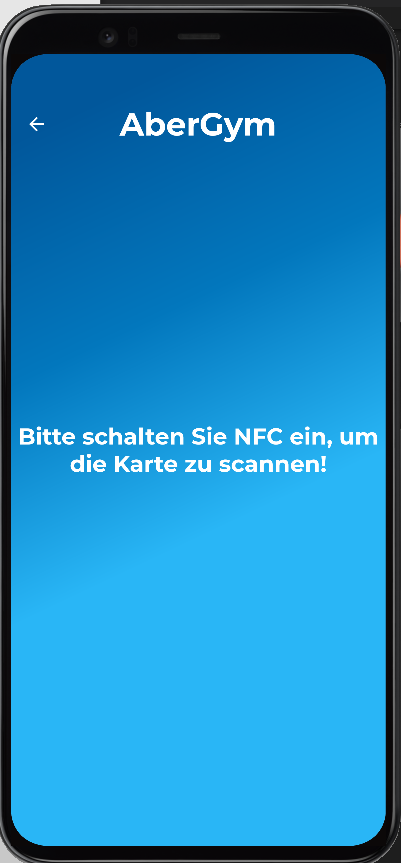
\includegraphics[scale=0.5]{pics/NFC.png}
        \caption{NFC}
    \end{figure}

    \newpage

    \section{Hauptmenü}
    \author{Antonio Kuvac}

    Im Hauptmenü kann der Benutzer*die Benutzerin sich den aktuellen Trainingsplan ansehen, den letzten Trainingsplan ansehen oder den Trainingsplan starten.

    \begin{figure}[H]
        \centering
        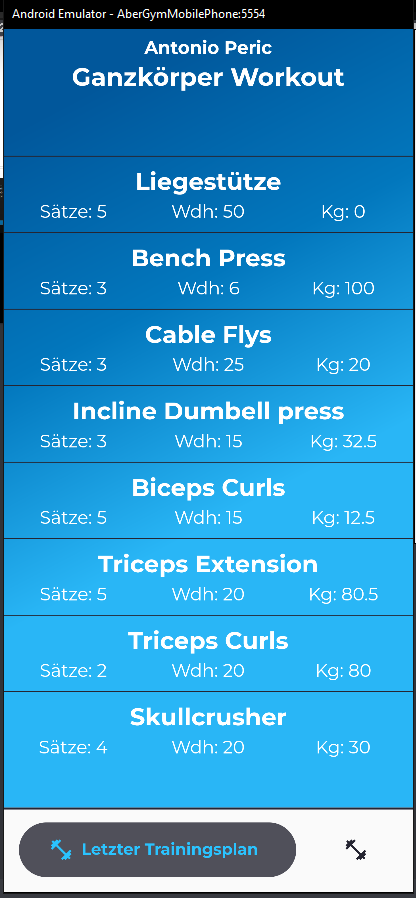
\includegraphics[scale=0.5]{pics/mainmenu.png}
        \caption{Hauptmenü}
    \end{figure}

    \pagebreak
    \subsection{Layout}


\begin{lstlisting}[caption=Layout Packages,label=lst:impl:frontend:qrcode]
import 'package:google_fonts/google_fonts.dart';
import 'package:google_nav_bar/google_nav_bar.dart';
\end{lstlisting}

Das Paket \texttt{googlefonts} ermöglicht die Verwendung von Google Fonts, während das Paket \texttt{googlenavbar} für die Erstellung der Navigationsleiste verwendet wird.
\\

\begin{lstlisting}[caption=LayoutState,label=lst:impl:frontend:qrcode]
class _LayoutState extends State<Layout> {
final bodies = [const SecondPage(), const HomePage()];
int currentIndex = 1;
Color lightblue = const Color.fromARGB(255, 42, 195, 255);
Color darkgrey = const Color.fromRGBO(37, 37, 50, 1);
\end{lstlisting}

Die Klasse \texttt{LayoutState} erbt von der \texttt{State<Layout>} Basisklasse und definiert einige Eigenschaften, wie die Liste der Seiten, den aktuellen ausgewählten Index und Farben für das Design der Navigationsleiste.
\\

\begin{lstlisting}[caption=Layout Scaffold-Widget,label=lst:impl:frontend:qrcode]
@override
Widget build(BuildContext context) {
return Scaffold(
body: bodies[currentIndex],
bottomNavigationBar: Stack(
\end{lstlisting}

Das \texttt{Scaffold}-Widget stellt das Grundgerüst für das Layout der App bereit. Der \texttt{body} wird durch den aktuellen ausgewählten Index in der \texttt{bodies}-Liste bestimmt. Die \texttt{bottomNavigationBar} ist ein \texttt{Stack}-Widget, das die Navigationsleiste und eine Linie oben auf der Navigationsleiste enthält.
\\

\begin{lstlisting}[caption=Navbar,label=lst:impl:frontend:qrcode]
children: [
Padding(
padding: const EdgeInsets.symmetric(horizontal: 15.0, vertical: 15),
child: GNav(
curve: Curves.easeOutSine,
color: darkgrey,
gap: 8,
iconSize: 25,
activeColor: lightblue,
tabBackgroundColor: darkgrey.withOpacity(0.8),
padding: const EdgeInsets.symmetric(vertical: 15, horizontal: 30),
duration: const Duration(milliseconds: 500),
tabs: [
GButton(
icon: Icons.fitness_center,
text: "Letzter Trainingsplan",
textStyle: GoogleFonts.montserrat(
color: lightblue,
fontSize: 16,
fontWeight: FontWeight.bold,
),
),
GButton(
icon: Icons.fitness_center,
text: "Heutiger Trainingsplan",
textStyle: GoogleFonts.montserrat(
color: lightblue,
fontSize: 16,
fontWeight: FontWeight.bold,
),
),
],
selectedIndex: currentIndex,
onTabChange: (index) {
    setState(() {
    currentIndex = index;
    });
    },
    ),
    ),
    Positioned(
    top: 0,
    left: 0,
    right: 0,
    child: Container(
    height: 2,
    color: darkgrey,
    ),
    ),
    ],
    ),
    );
    }
    }
}
\end{lstlisting}
    
    Die \texttt{GNav}-Komponente erstellt die Navigationsleiste und definiert deren Aussehen und Verhalten. Die Navigationsleiste besteht aus zwei \texttt{GButton}-Widgets, die jeweils ein Icon und einen Text enthalten. Der Stil des Textes wird mit dem GoogleFonts-Paket festgelegt. Die \texttt{selectedIndex}-Eigenschaft gibt den ausgewählten Index der Navigationsleiste an, und die \texttt{onTabChange}-Eigenschaft ist eine Funktion, die den aktuellen Index aktualisiert, wenn der Benutzer*die Benutzerin eine andere Registerkarte auswählt.
    

    \subsection{HomePage}
    \author{Antonio Kuvac}

\begin{lstlisting}[caption=Trainingsplan Logik,label=lst:impl:frontend:qrcode]
final prefs = await SharedPreferences.getInstance();
int? amountrows = prefs.getInt('amountrows');
int countTrue = 0;

        if (amountrows != null) {
          for (int i = 0; i < amountrows; i++) {
            if (prefs.getBool('finishedExcersice_$i') == true) {
              countTrue++;
            }
          }
          if (countTrue == amountrows) {
            for (int i = 0; i < amountrows; i++) {
              prefs.remove('finishedExcersice_$i');
            }
          }
        }

        _navigateToNextScreen(context);
\end{lstlisting}

Innerhalb der \texttt{onPressed}-Funktion wird die Logik für das Starten des Trainingsplans und das Verwalten der SharedPreferences implementiert. Die SharedPreferences-Instanz wird abgerufen, und die Anzahl der Zeilen und die Anzahl der abgeschlossenen Übungen werden verwaltet. Wenn alle Übungen abgeschlossen sind, werden die SharedPreferences-Einträge entfernt. Schließlich wird die Funktion \texttt{navigateToNextScreen} aufgerufen, um zur nächsten Seite zu navigieren.
\\

\begin{lstlisting}[caption=Trainingsplan starten Knopf,label=lst:impl:frontend:qrcode]
style: ElevatedButton.styleFrom(
backgroundColor: darkgrey.withOpacity(0.8),
shape: const RoundedRectangleBorder(
borderRadius: BorderRadius.only(
topRight: Radius.circular(0.0),
topLeft: Radius.circular(0.0),
),
),
),
child: SizedBox(
height: 216,
child: Column(
),
),
\end{lstlisting}

Für den Trainingsplan Starten Knopf wurde der Hintergrund des \texttt{ElevatedButton}-Widgets mit einer leicht transparenten dunkelgrauen Farbe festgelegt. Die Form des Buttons ist ein rechteckiges Widget mit abgerundeten Ecken an der Oberseite. Der Inhalt des Buttons besteht aus einer \texttt{SizedBox} mit einer festen Höhe und einer \texttt{Column}, die die Text- und Icon-Widgets enthält.
\\


\begin{lstlisting}[caption=HomePage Navigation,label=lst:impl:frontend:qrcode]
void _navigateToNextScreen(BuildContext context) {
Navigator.of(context)
.push(MaterialPageRoute(builder: (context) => const LayoutTDL()));
}
\end{lstlisting}

Die Navigationsfunktion \texttt{navigateToNextScreen} wird definiert, um zur nächsten Seite zu navigieren.Die Funktion \texttt{navigateToNextScreen} akzeptiert ein \texttt{BuildContext}-Objekt und verwendet den \texttt{Navigator} zum Navigieren zur nächsten Seite, die durch das \texttt{LayoutTDL}-Widget dargestellt wird.

\pagebreak
    \subsection{SecondPage}
    \author{Antonio Kuvac}

    \begin{lstlisting}[caption=Second Page,label=lst:impl:frontend:qrcode]
        class SecondPage extends StatelessWidget {
  const SecondPage({super.key});

  @override
  Widget build(BuildContext context) {
    return SqlTable(version: 0);
  }
}
    \end{lstlisting}

    Die SecondPage Methode lädt, wenn die "Letzter Trainingsplan" Seite ausgewählt wird, aus der Datenbank den letzten Trainingsplan. 

    

    \section{To-Do-Liste}
    \author{Antonio Kuvac}

    Die To-Do-Liste ist eine interaktive Liste aus Übungen die im Trainingsplan enthalten sind. Durch das Auswählen einer Übung in dieser Liste, wird man an die Satzzähler Seite weitergeleitet. Wenn man eine Übung abgeschlossen hat, wird die Übung in der Liste ausgegraut und an letzter Stelle der Liste verschoben.

    \begin{figure}[H]
        \centering
        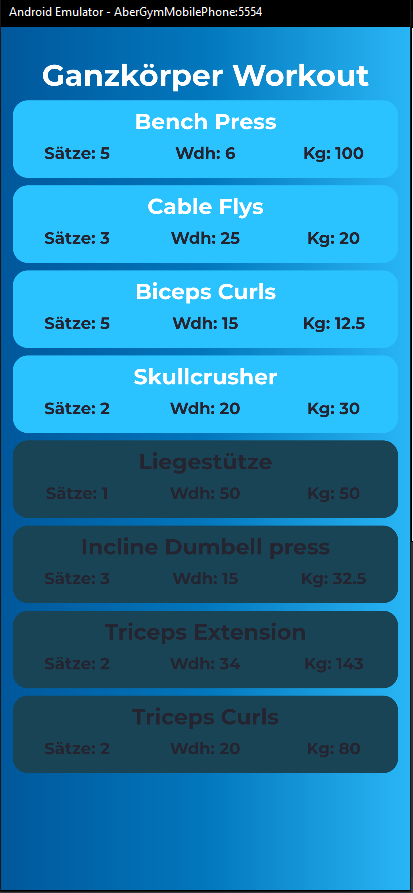
\includegraphics[scale=0.3]{pics/To-Do-Liste.png}
        \caption{To-Do-Liste}
    \end{figure}
    
    \pagebreak
    \begin{lstlisting}[caption=To-Do-Liste Trainingsplan Variablen,label=lst:impl:frontend:qrcode]
    late String wname = "";
    late List<String> wereps = [];
    late List<String> wesets = [];
    late List<String> weweight = [];
    late List<String> ename = [];
    late int amountrows = 0;
    final Color lightblue = const Color.fromARGB(255, 42, 195, 255);
    final Color darkgrey = const Color.fromRGBO(37, 37, 50, 1);
    List<bool> finishedExcersiceList = [];
    int counter = 0;
    bool finished = false;
    \end{lstlisting}
    
    Diese Variablen enthalten Informationen über die Übungen, die Anzahl der Zeilen, Farben und ob eine Übung abgeschlossen ist oder nicht.
    \\
    
    
    \begin{lstlisting}[caption=To-Do-Liste get Methode,label=lst:impl:frontend:qrcode]
        void getData() async {
            final prefs = await SharedPreferences.getInstance();
            wname = prefs.getString('wname')!;
            wereps = prefs.getStringList('wereps')!;
            wesets = prefs.getStringList('wesets')!;
            weweight = prefs.getStringList('weweight')!;
            ename = prefs.getStringList('ename')!;
            amountrows = prefs.getInt('amountrows')!;
        
            for (int i = 0; i < amountrows; i++) {
              if (prefs.get('finishedExcersice_$i') == true) {
                finishedExcersiceList.add(true);
                setState(() {
                  counter++;
                });
              } else {
                finishedExcersiceList.add(false);
              }
            }
            if (counter == amountrows) {
              setState(() {
                finished = true;
              });
            }
            setState(() {
              wname = wname;
              wereps = wereps;
              wesets = wesets;
              wesets = wesets;
              weweight = weweight;
              ename = ename;
              amountrows = amountrows;
            });
          }
    \end{lstlisting}
    
    Die Methode \texttt{getData} liest die Daten aus SharedPreferences und aktualisiert die Zustände der ToDoList-Klasse. 
    
    \pagebreak
    \begin{lstlisting}[caption=To-Do-Liste Item Methode,label=lst:impl:frontend:qrcode]
        Container toDoListItem(int i, bool isFinished) {
            return Container(
              height: 78,
              margin: const EdgeInsets.only(
                top: 3.8,
                right: 12,
                left: 12,
                bottom: 3.8,
              ),
              decoration: isFinished
                  ? BoxDecoration(
                      borderRadius: BorderRadius.circular(15.0),
                      color: const Color.fromARGB(255, 25, 68, 85),
                    )
                  : BoxDecoration(
                      borderRadius: BorderRadius.circular(15.0),
                      color: lightblue,
                    ),
              child: Column(
                children: [
                  Container(
                    padding: const EdgeInsets.all(8.0),
                    child: Text(
                      (ename.isNotEmpty ? ename[i].toString() : ""),
                      textScaleFactor: 2,
                      style: isFinished
                          ? GoogleFonts.montserrat(
                              fontSize: 11,
                              color: darkgrey,
                              fontWeight: FontWeight.bold,
                            )
                          : GoogleFonts.montserrat(
                              fontSize: 11,
                              color: Colors.white,
                              fontWeight: FontWeight.bold,
                            ),
                      textAlign: TextAlign.center,
                    ),
                  ),
                  Table(
                    children: [
                      TableRow(
                        children: [
                          Center(
                            child: Text(
                              (wesets.isNotEmpty
                                  ? 'Saetze: ${wesets[i].toString()}'
                                  : ""),
                              textScaleFactor: 1.5,
                              style: GoogleFonts.montserrat(
                                fontSize: 11,
                                color: darkgrey,
                                fontWeight: FontWeight.bold,
                              ),
                            ),
                          ),
                          Center(
                            child: Text(
                              (wereps.isNotEmpty ? 'Wdh: ${wereps[i].toString()}' : ""),
                              textScaleFactor: 1.5,
                              style: GoogleFonts.montserrat(
                                fontSize: 11,
                                color: darkgrey,
                                fontWeight: FontWeight.bold,
                              ),
                            ),
                          ),
                          Center(
                            child: Text(
                              (weweight.isNotEmpty
                                  ? 'Kg: ${weweight[i].toString()}'
                                  : ""),
                              textScaleFactor: 1.5,
                              style: GoogleFonts.montserrat(
                                fontSize: 11,
                                color: darkgrey,
                                fontWeight: FontWeight.bold,
                              ),
                            ),
                          ),
                        ],
                      ),
                    ],
                  ),
                ],
              ),
            );
          }
        
    \end{lstlisting}

    Die \texttt{toDoListItem}-Methode erstellt ein individuelles Aufgabenlisten-Element basierend auf einem gegebenen Index und ob es abgeschlossen ist oder nicht.

    \section{Satzzähler}
    \author{Antonio Kuvac}

    Der Satzzähler ermöglicht es beim Trainieren, die Sätze der aktuell ausgewählten Übung mitzuzählen und somit die Übung abzuschließen.

    \begin{figure}[H]
        \centering
        \includegraphics[scale=0.3]{pics/Satzzähler.png}
        \caption{Satzzähler}
    \end{figure}

    \begin{lstlisting}[caption=SetCounter,label=lst:impl:frontend:qrcode]
        class SetCounter extends StatefulWidget {
        int index = 0;
        SetCounter({super.key, required this.index});
        
        @override
        State<SetCounter> createState() => _SetCounterState(index);
        }
        \end{lstlisting}
        
        Die Klasse SetCounter erbt von StatefulWidget und nimmt den Parameter index entgegen. Dieser Index gibt die Position der aktuellen Übung in der Liste an. Der Konstruktor der Klasse speichert den Index und übergibt ihn an den State der Klasse, SetCounterState.
        \\
        
        \begin{lstlisting}[caption=SetCounterState,label=lst:impl:frontend:qrcode]
        class _SetCounterState extends State<SetCounter> {
        int index = 0;
        late List<String> werepsList = [];
        late List<String> wesetsList = [];
        late List<String> weweightList = [];
        late List<String> enameList = [];
        String wereps = "";
        String wesets = "";
        String weweight = "";
        String ename = "";
        Color lightblue = const Color.fromARGB(255, 42, 195, 255);
        Color darkgrey = const Color.fromRGBO(37, 37, 50, 1);
        int counter = 0;
        late bool finishedExcersice;
        double? fontSizeRows = 13;
        double? fontPixelsRows = 1.5;
        
        _SetCounterState(this.index);
        }
        \end{lstlisting}
        
        Die Klasse SetCounterState speichert den index und verwaltet die Zustände der App. Es gibt verschiedene Zustandsvariablen für die Anzahl der Wiederholungen, Sätze, das Gewicht und den Namen der Übung. 
        \\
        
        
        \begin{lstlisting}[caption=Increase Counter Funktion,label=lst:impl:frontend:qrcode]
        void increaseCounter() async {
        final prefs = await SharedPreferences.getInstance();
        setState(() => counter++);
        if (counter > int.parse(wesets)) {
        finishedExcersice = true;
        prefs.setBool('finishedExcersice$index', finishedExcersice);
        }
        }
        \end{lstlisting}

        Die increaseCounter-Funktion erhöht den Satzzähler und aktualisiert die Benutzeroberfläche. Wenn die Anzahl der abgeschlossenen Sätze größer ist als die vorgegebene Anzahl der Sätze, wird die Variable finishedExcersice auf true gesetzt und in den SharedPreferences gespeichert.
        \\

        \begin{lstlisting}[caption=initState,label=lst:impl:frontend:qrcode]
            @override
            void initState() {
            super.initState();
            getData();
            }
            \end{lstlisting}
            \pagebreak
            Die initState()-Funktion wird aufgerufen, wenn der Zustand des Widgets initialisiert wird. Hier wird die Funktion getData() aufgerufen, um die Daten für die aktuelle Übung zu laden.
            \\
            
            \begin{lstlisting}[caption=GestureDetector,label=lst:impl:frontend:qrcode]
                GestureDetector(
                    onTap: _increaseCounter,
                    child: Container(
                      padding: const EdgeInsets.only(top: 65),
                      margin: const EdgeInsets.all(50.0),
                      width: 300.0,
                      height: 300.0,
                      decoration: BoxDecoration(
                        gradient: LinearGradient(
                          begin: Alignment.centerLeft,
                          colors: [
                            Colors.lightBlue[900]!,
                            Colors.lightBlue[800]!,
                            Colors.lightBlue[400]!,
                          ],
                        ),
                        shape: BoxShape.circle,
                      ),
                      child: Column(
                        children: [
                          Text(
                            '$counter/$wesets',
                            style: GoogleFonts.montserrat(
                              color: Colors.white,
                              fontSize: 100,
                            ),
                          ),
                          Text(
                            "Erledigte Saetze",
                            style: GoogleFonts.montserrat(
                              color: Colors.white,
                              fontSize: 25,
                              fontWeight: FontWeight.bold,
                            ),
                          ),
                        ],
                      ),
                    ),
                  ),
            \end{lstlisting}
            
            Ein GestureDetector wird verwendet, um auf Berührungen des Benutzers zu reagieren und den Satzzähler entsprechend zu erhöhen. Wenn der Benutzer auf den Container tippt, wird die increaseCounter-Funktion aufgerufen.
            \\

            \begin{lstlisting}[caption=GestureDetector zum Schluss,label=lst:impl:frontend:qrcode]
                GestureDetector(
                    onTap: () {
                      Navigator.push(
                        context,
                        MaterialPageRoute(
                          builder: (context) => const ToDoList(),
                        ),
                      );
                    },
                    child: Container(
                      padding: const EdgeInsets.only(top: 65),
                      margin: const EdgeInsets.all(50.0),
                      width: 300.0,
                      height: 300.0,
                      decoration: BoxDecoration(
                        gradient: LinearGradient(
                          begin: Alignment.centerLeft,
                          colors: [
                            Colors.lightBlue[900]!,
                            Colors.lightBlue[800]!,
                            Colors.lightBlue[400]!,
                          ],
                        ),
                        shape: BoxShape.circle,
                      ),
                      child: Column(
                        children: [
                          InkWell(
                            onTap: () {
                              Navigator.push(
                                context,
                                MaterialPageRoute(
                                  builder: (context) => const ToDoList(),
                                ),
                              );
                            },
                            child: Column(
                              children: <Widget>[
                                Text(
                                  "Uebung",
                                  style: GoogleFonts.montserrat(
                                    color: Colors.white,
                                    fontSize: 70,
                                  ),
                                ),
                                Text(
                                  "Fertig",
                                  style: GoogleFonts.montserrat(
                                    color: Colors.white,
                                    fontSize: 65,
                                  ),
                                ),
                              ],
                            ),
                          ),
                        ],
                      ),
                    ),
                  ),
            \end{lstlisting}
            
            Wenn die Übung abgeschlossen ist (wenn die Anzahl der abgeschlossenen Sätze gleich oder größer als die vorgegebene Anzahl ist), wird ein anderer GestureDetector und Container angezeigt, der dem Benutzer signalisiert, dass die Übung beendet ist. Bei einem Tippen auf den Container wird der Benutzer zur ToDoList-Seite weitergeleitet.
            \\

    \section{Trainingplan bearbeiten}
    \author{Antonio Kuvac}

    Durch langes gedrückt halten einer Übung in der To-Do-Liste wird die Bearbeitungsseite geöffnet und die ausgewählte Übung kann bearbeitet werden. Es können die Wiederholungen, die Sätze und das Gewicht geändert werden, um während des Trainings flexibel auf eigene Wünsche das Training anpassen zu können.

    \begin{figure}[H]
        \centering
        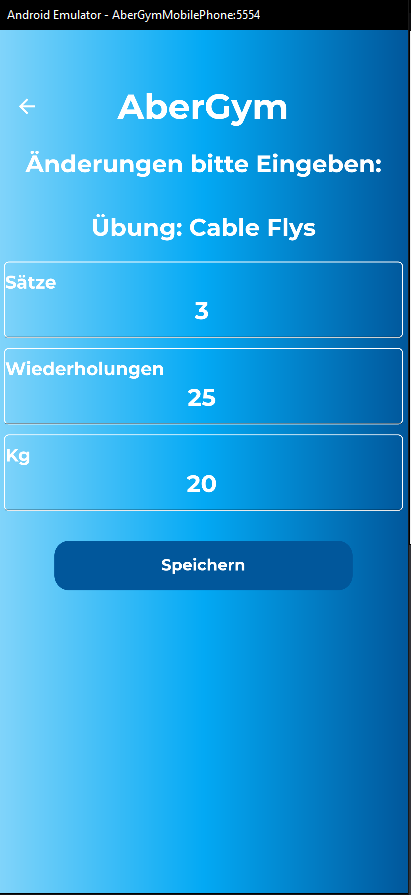
\includegraphics[scale=0.3]{pics/Bearbeiten.png}
        \caption{Trainingplan bearbeiten}
    \end{figure}

    \begin{lstlisting}[caption=Bearbeiten Index,label=lst:impl:frontend:qrcode]
        class UpdateExcersice extends StatefulWidget {
        int index = 0;
        UpdateExcersice({super.key, required this.index});
        
        @override
        State<UpdateExcersice> createState() => _UpdateExcersiceState(index);
        }
        \end{lstlisting}
        
        Die UpdateExcersice-Klasse erbt von StatefulWidget und speichert den index der aktuellen Übung. Der Konstruktor nimmt den index als erforderliches Argument an und übergibt diesen an die UpdateExcersiceState-Klasse.
        \\
         

        \begin{lstlisting}[caption=Bearbeiten UpdateExcersiceState,label=lst:impl:frontend:qrcode]
              class _UpdateExcersiceState extends State<UpdateExcersice> {
                int index = 0;
                late List<String> werepsList = [];
                late List<String> wesetsList = [];
                late List<String> weweightList = [];
                late List<String> enameList = [];
                String wereps = "";
                String wesets = "";
                String weweight = "";
                String ename = "";
                Color lightblue = const Color.fromARGB(255, 42, 195, 255);
                Color darkgrey = const Color.fromRGBO(37, 37, 50, 1);
                String _sets = '';
                String _reps = '';
                String _kg = '';
                final setsController = TextEditingController();
                final repsController = TextEditingController();
                final kgController = TextEditingController();
              
                _UpdateExcersiceState(this.index);
              
                void getData() async {
                  final prefs = await SharedPreferences.getInstance();
                  werepsList = prefs.getStringList('wereps')!;
                  wesetsList = prefs.getStringList('wesets')!;
                  weweightList = prefs.getStringList('weweight')!;
                  enameList = prefs.getStringList('ename')!;
              
                  setState(() {
                    wereps = werepsList[index];
                    wesets = wesetsList[index];
                    weweight = weweightList[index];
                    ename = enameList[index];
                    setsController.text = wesets;
                    repsController.text = wereps;
                    kgController.text = weweight;
                  });
                }}
        \end{lstlisting}
        
        Die UpdateExcersiceState-Klasse erweitert die State-Klasse für das UpdateExcersice-Widget. Innerhalb dieser Klasse werden verschiedene Variablen und Methoden definiert, um Daten zu laden, zu speichern und die Benutzeroberfläche aufzubauen.
        \\
        

        \begin{lstlisting}[caption=Bearbeiten initState getData,label=lst:impl:frontend:qrcode]
        void initState() {
        super.initState();
        getData();
        }
        \end{lstlisting}
        
        Die initState-Methode wird aufgerufen, wenn der Zustand des Widgets initialisiert wird. Hier wird die getData-Methode aufgerufen, um die aktuellen Daten der Übung zu laden.
        \\

        \begin{lstlisting}[caption=Bearbeiten Build,label=lst:impl:frontend:qrcode]
        @override
        Widget build(BuildContext context) {
            @override
            Widget build(BuildContext context) {
              return Scaffold(
                extendBodyBehindAppBar: true,
                appBar: AppBar(
                  title: Text(
                    'AberGym',
                    style: GoogleFonts.montserrat(
                      fontSize: 35,
                      color: Colors.white,
                      fontWeight: FontWeight.bold,
                    ),
                  ),
                  backgroundColor: Colors.transparent,
                  centerTitle: true,
                  elevation: 0,
                ),
                body: Container(
                  padding: const EdgeInsets.only(top: 110),
                  decoration: BoxDecoration(
                    gradient: LinearGradient(
                      begin: Alignment.centerLeft,
                      colors: [
                        Colors.lightBlue[200]!,
                        Colors.lightBlue[500]!,
                        Colors.lightBlue[900]!,
                      ],
                    ),
                  ),
                  child: Center(
                    child: Column(
                      children: [
                        Container(
                          padding: const EdgeInsets.all(10.0),
                          child: Text(
                            "Aenderungen bitte Eingeben:",
                            style: GoogleFonts.montserrat(
                              fontSize: 24,
                              color: Colors.white,
                              fontWeight: FontWeight.bold,
                            ),
                            textAlign: TextAlign.center,
                          ),
                        ),
                        Container(
                          padding: const EdgeInsets.only(bottom: 15.0, top: 25),
                          child: Text(
                            'Uebung: $ename',
                            style: GoogleFonts.montserrat(
                              fontSize: 24,
                              color: Colors.white,
                              fontWeight: FontWeight.bold,
                            ),
                            textAlign: TextAlign.center,
                          ),
                        ),
                        // Textfeld 1
                        Container(
                          margin: const EdgeInsets.all(5),
                          decoration: BoxDecoration(
                            borderRadius: BorderRadius.circular(5),
                            border: Border.all(color: Colors.white),
                          ),
                          child: TextField(
                            keyboardType: TextInputType.number,
                            decoration: InputDecoration(
                              labelText: 'Saetze',
                              labelStyle: GoogleFonts.montserrat(
                                fontSize: 24,
                                color: Colors.white,
                                fontWeight: FontWeight.bold,
                              ),
                            ),
                            controller: setsController,
                            onChanged: (value) {
                              _saveInput();
                            },
                            onTap: () {
                              setsController.clear();
                            },
                            textAlign: TextAlign.center,
                            style: GoogleFonts.montserrat(
                              fontSize: 24,
                              color: Colors.white,
                              fontWeight: FontWeight.bold,
                            ),
                          ),
                        ),
                        // Textfeld 2
                        Container(
                          margin: const EdgeInsets.all(5),
                          decoration: BoxDecoration(
                            borderRadius: BorderRadius.circular(5),
                            border: Border.all(color: Colors.white),
                          ),
                          child: TextField(
                            keyboardType: TextInputType.number,
                            decoration: InputDecoration(
                              labelText: 'Wiederholungen',
                              labelStyle: GoogleFonts.montserrat(
                                fontSize: 24,
                                color: Colors.white,
                                fontWeight: FontWeight.bold,
                              ),
                            ),
                            controller: repsController,
                            onChanged: (value) {
                              _saveInput();
                            },
                            onTap: () {
                              repsController.clear();
                            },
                            textAlign: TextAlign.center,
                            style: GoogleFonts.montserrat(
                              fontSize: 24,
                              color: Colors.white,
                              fontWeight: FontWeight.bold,
                            ),
                          ),
                        ),
                        // Textfeld 3
                        Container(
                          margin: const EdgeInsets.all(5),
                          decoration: BoxDecoration(
                            borderRadius: BorderRadius.circular(5),
                            border: Border.all(color: Colors.white),
                          ),
                          child: TextField(
                            keyboardType: TextInputType.number,
                            decoration: InputDecoration(
                              labelText: 'Kg',
                              labelStyle: GoogleFonts.montserrat(
                                fontSize: 24,
                                color: Colors.white,
                                fontWeight: FontWeight.bold,
                              ),
                            ),
                            controller: kgController,
                            onChanged: (value) {
                              _saveInput();
                            },
                            onTap: () {
                              kgController.clear();
                            },
                            textAlign: TextAlign.center,
                            style: GoogleFonts.montserrat(
                              fontSize: 24,
                              color: Colors.white,
                              fontWeight: FontWeight.bold,
                            ),
                          ),
                        ),
                        GestureDetector(
                          onTap: () async {
                            await saveInputInCache();
                            Navigator.push(
                              context,
                              PageTransition(
                                type: PageTransitionType.leftToRight,
                                child: const LayoutTDL(),
                              ),
                            );
                          },
                          child: Container(
                            margin: const EdgeInsets.only(top: 25),
                            width: 300,
                            height: 50,
                            decoration: BoxDecoration(
                              color: Colors.lightBlue[900]!,
                              borderRadius: BorderRadius.circular(15),
                            ),
                            child: Row(
                              mainAxisAlignment: MainAxisAlignment.center,
                              children: [
                                Text(
                                  'Speichern',
                                  style: GoogleFonts.montserrat(
                                    fontSize: 16,
                                    color: Colors.white,
                                    fontWeight: FontWeight.bold,
                                  ),
                                ),
                              ],
                            ),
                          ),
                        ),
                      ],
                    ),
                  ),
                ),
              );
            }
        }
        \end{lstlisting}
        
        Die build-Methode erstellt die Benutzeroberfläche für das Widget. In dieser Methode wird ein Scaffold-Widget verwendet, um die grundlegende Struktur der App zu definieren. Die Benutzeroberfläche besteht aus mehreren Eingabefeldern und Schaltflächen, die den Benutzer*innen ermöglichen, ihre Änderungen einzugeben und zu speichern.
        \\
        

        \begin{lstlisting}[caption=Bearbeiten saveInput,label=lst:impl:frontend:qrcode]
        void _saveInput() {
        setState(() {
        _sets = setsController.text;
        _reps = repsController.text;
        _kg = kgController.text;
        });
        }
        \end{lstlisting}
        
        Die saveInput-Methode speichert die Benutzereingaben in den entsprechenden Variablen. Diese Methode wird aufgerufen, wenn der Inhalt eines der Eingabefelder geändert wird.
        \\
        

        \begin{lstlisting}[caption=Bearbeiten saveInputInCache,label=lst:impl:frontend:qrcode]
            Future<void> saveInputInCache() async {
                  await conn.connect();
                  await conn.execute(
                    'UPDATE WorkoutExercise we JOIN Exercise e ON we.exercise_id = e.id SET we.`sets` = :sets, we.weight = :kg, we.reps = :reps WHERE e.name = :name AND we.workoutplan_id = (SELECT MAX(id) FROM Workoutplan)',
                    {"sets": _sets, "kg": _kg, "reps": _reps, "name": ename},
                  );
                  wesetsList[index] = _sets;
                  weweightList[index] = _kg;
                  werepsList[index] = _reps;
                  final prefs = await SharedPreferences.getInstance();
            
                  await prefs.remove('wesets');
                  await prefs.remove('weweight');
                  await prefs.remove('wereps');
            
                  await prefs.setStringList('wesets', wesetsList);
                  await prefs.setStringList('weweight', weweightList);
                  await prefs.setStringList('wereps', werepsList);
            
                  conn.close();
                }
        \end{lstlisting}
        
        Die saveInputInCache-Methode speichert die Benutzereingaben in den SharedPreferences und aktualisiert die Datenbank. Diese Methode wird aufgerufen, wenn der Benutzer auf die Schaltfläche "Speichern" tippt.